%\usepackage{cleveref}
\chapter{Results}

\label{ch:results}

\section{ATLAS\textsuperscript{3D}}
Initially, the algorithm was trained using the $\lambda_{Re}$ to predict the FS classification since they were related directly according to ref{eq:2.4}
(NEED TO FIX REFERENCING EQUATIONS). Promisingly, the classifier was 100\% successful in its predictions. Training was then performed using the Se\'rsic index of the single fit, n, and achieved success of 71\% which exactly matched the probability of randomly selecting the answer given by the binomial probability distribution which is necessary due to the binomial nature of the outcome with differing sizes of the two populations, given by\cite{simmons_2016}:
\begin{equation}
P(k successes in n trials) = \binom{n}{k}p^{k}q^{n-k}
\end{equation}
where $n$ is the number of trials, $k$ is the number of successes, $n-k$ is the number of failures, $p$ is the probability of success in one trial and $q=1-p$ is probability of failure in one trial. This indicates that the algorithm failed in its attempt to predict the rotation based on se\'rsic index alone. This is surprising given the morphological importance of this parameter, but maybe due to...\\
When we look at the D/T dependence of the $\lambda_{Re}$ value, we see a more promising separation of the two populations, with a value of D/T $\approx 0.28$ producing a low level of impurity. This parameter was identified as the most promising by \cite{Krajnovic2013}[p1790].
\begin{figure}[h]
	\caption{The separation between the two populations is more pronounced here. The galaxies with D/T = 0 have no exponential discs.
	}
	\centering
	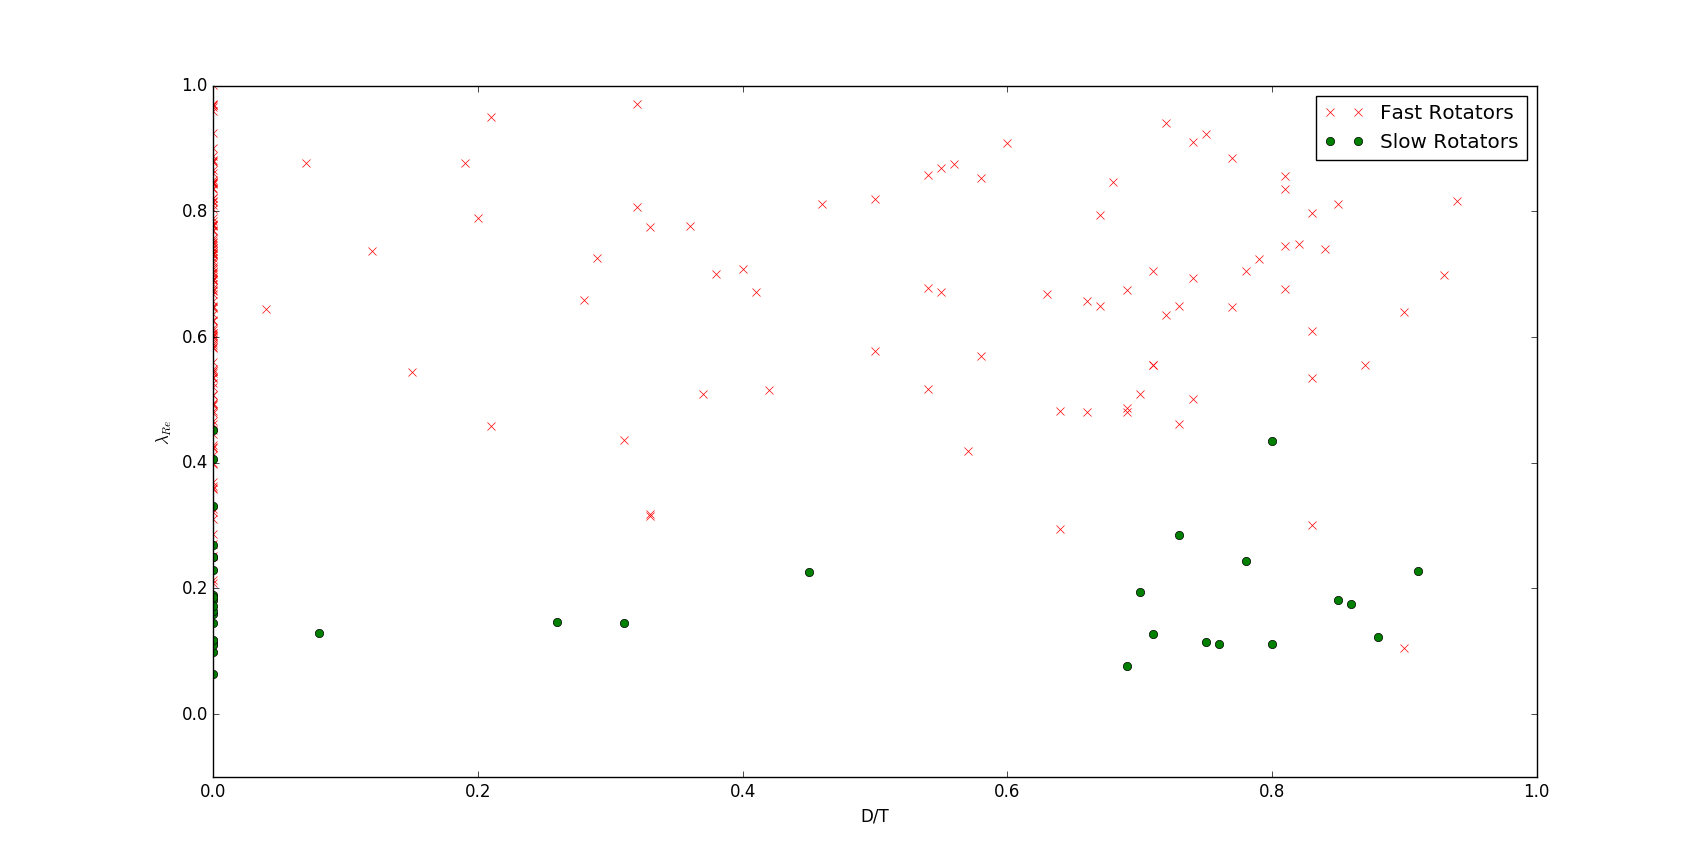
\includegraphics[width=\textwidth]{DT_lamre.png}
	\label{fig:dtlamre}
\end{figure}
The algorithm was then trained using D/T, improving the success rate to 81\%. Interestingly, when we evaluate the success of the decision tree classifier for those galaxies with no exponential disk component, where D/T$\lessapprox $0.05, we find that the decision tree is still able to correctly classify the majority of galaxies.